%% ----------------------------------------------------------------
%% Introduction
%% ----------------------------------------------------------------
%!TeX root = subfile
\label{chapter:introduction}
\documentclass[../main.tex]{subfiles}
% ----------------------------------------------------------------
\begin{document}
Marine risers are long flexible cylindrical structures that extract oil and gas from subsea oil fields to the surface (\fref{fig:riser}).
Under ocean currents, they are exposed to vortex-induced vibrations (VIV), a phenomenon arising in external flows past solid bodies which is particularly important for long, thin and flexible body shapes.
An alternate shedding of vortices from the upper and the lower sides of the riser circular section, a.k.a von-K\'{a}rm\'{a}n vortex street, creates an unsteady asymmetrical load pattern that stimulates a vibrational state of the riser.
This endangers the structure to severe fatigue reducing its lifespan significantly.
Besides the VIV phenomenon, wake-induced vibrations (WIV) also come into the picture for structures composed by multiple risers, adding notable complexity to the problem.
WIV, or wake galloping, takes place when one body is exposed to the non-uniform wake of another one.
This phenomenon can cause larger structural displacements compared to the VIV response of the isolated body \citep{Assi2014}.

\begin{figure}[t]
\centering
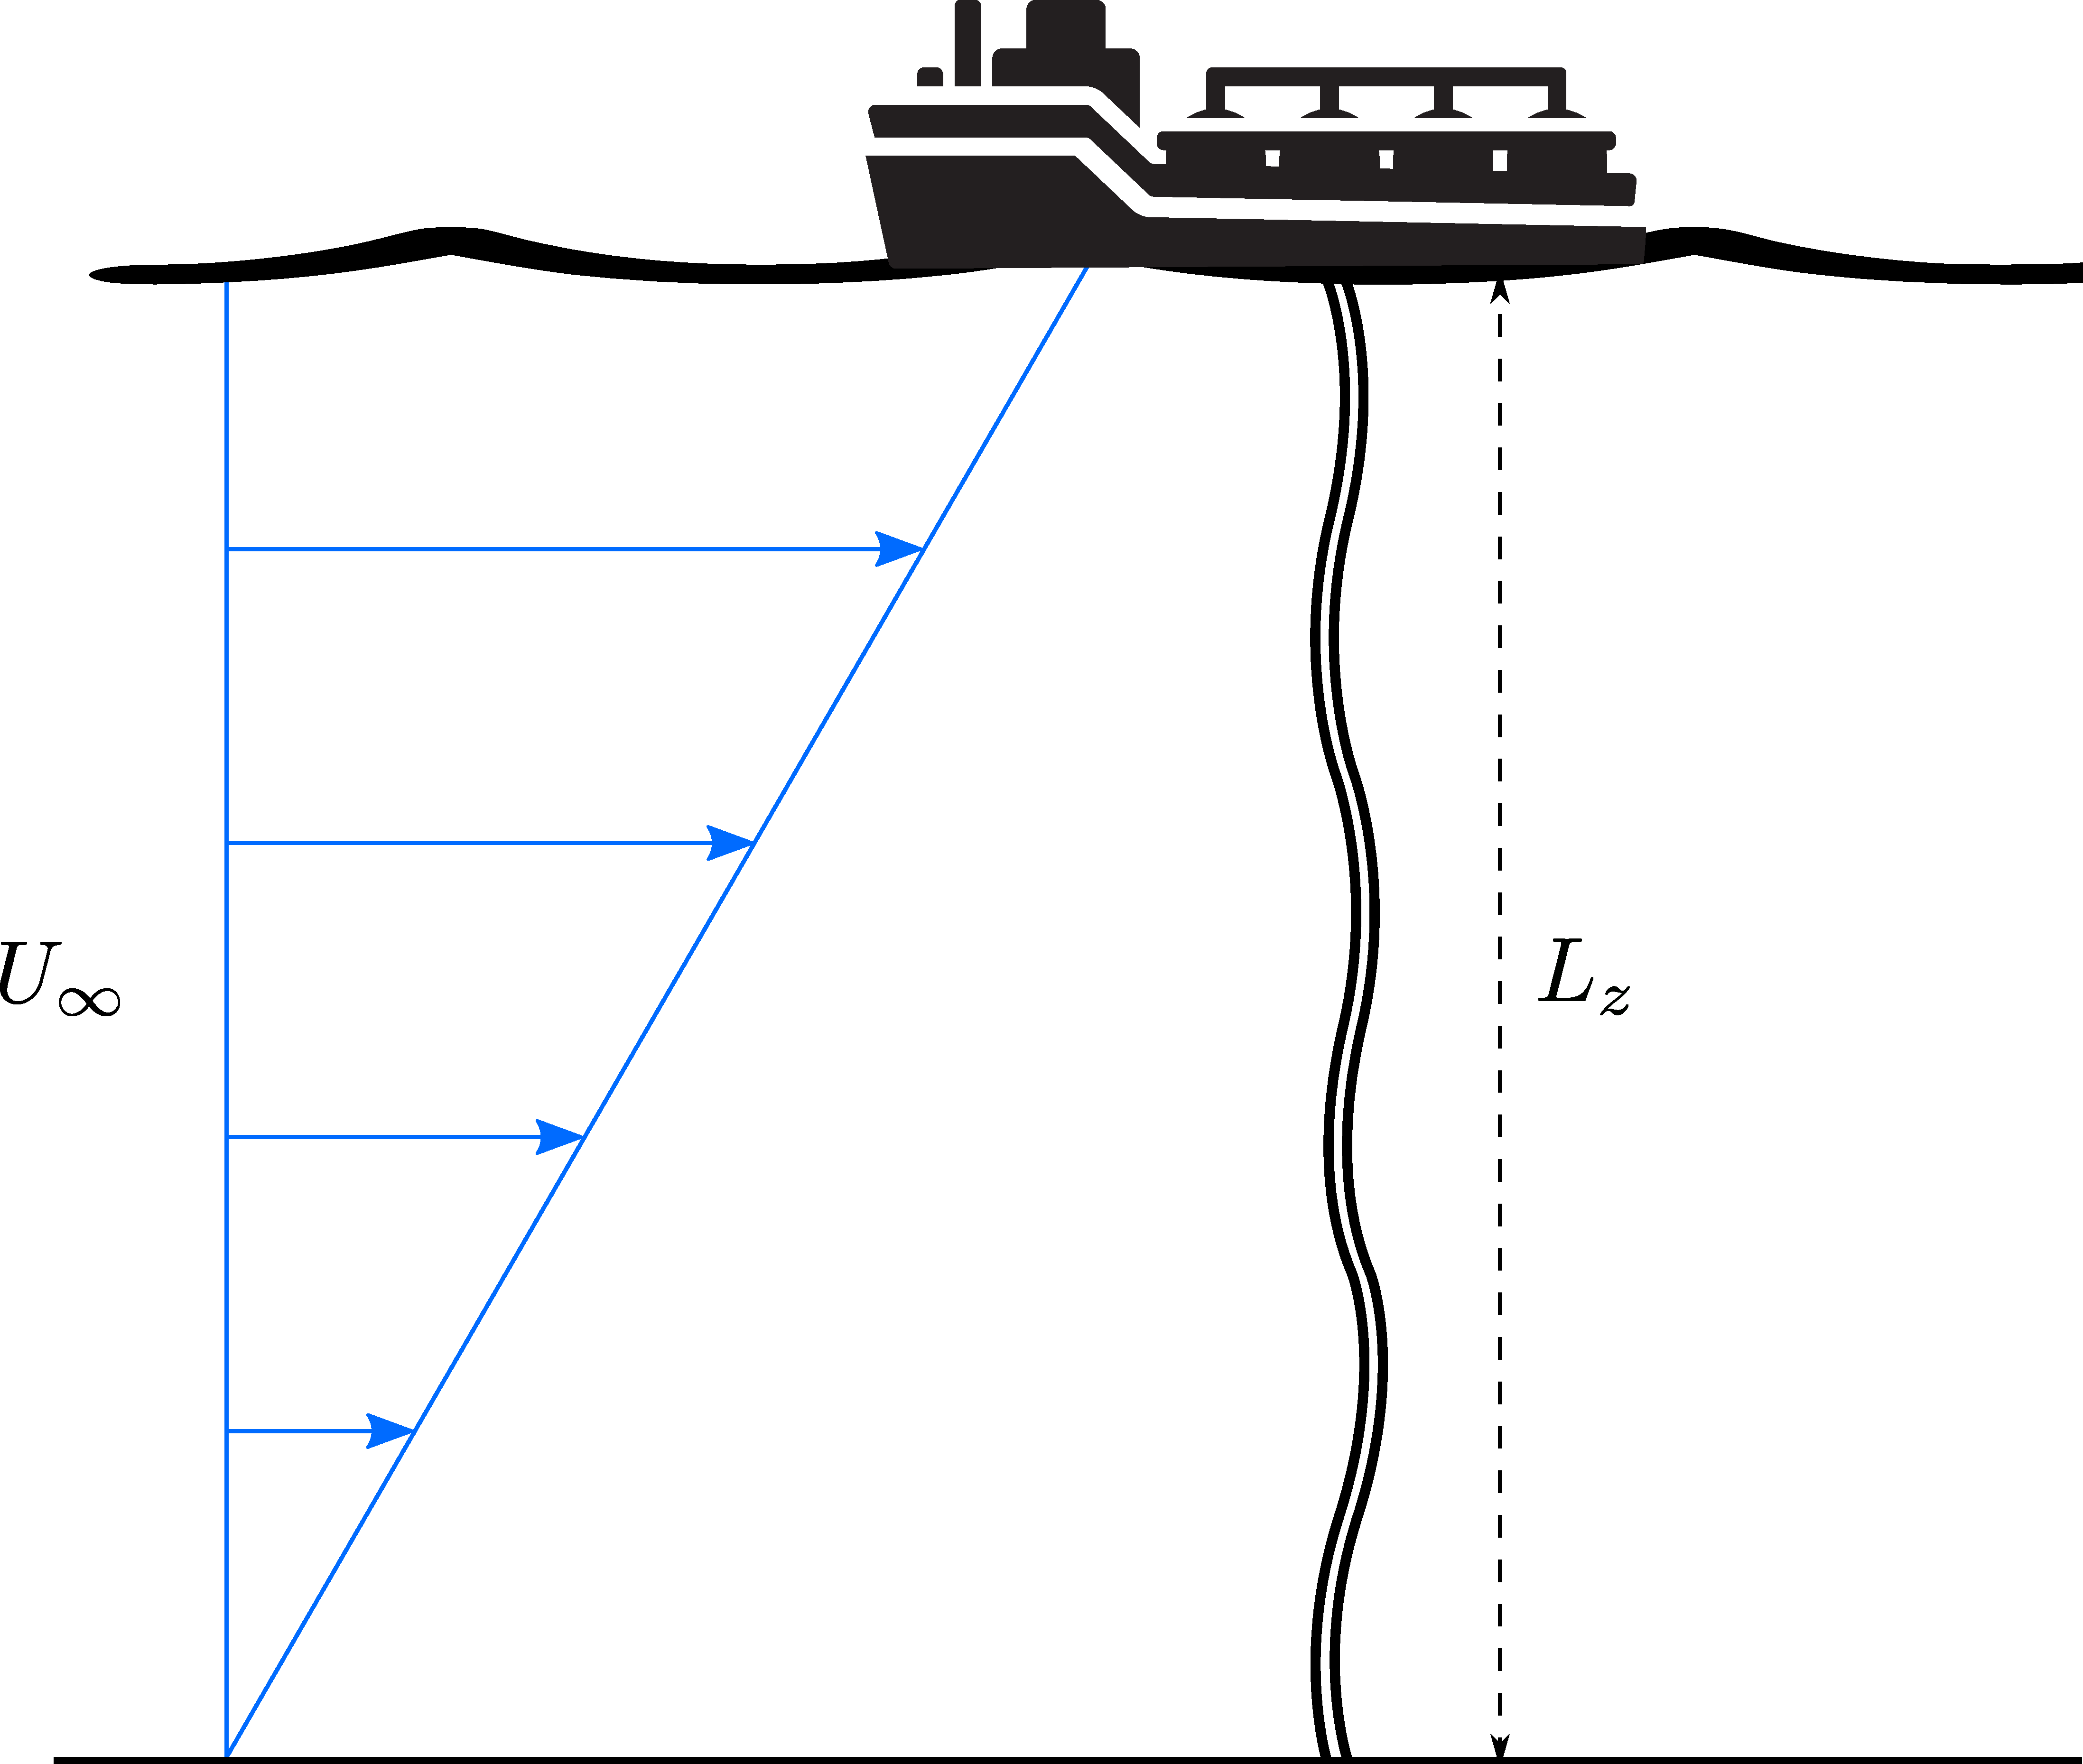
\includegraphics[width=0.5\linewidth]{chapter1/riser}
\caption{Sketch of a marine riser exposed to a sheared onset current profile.}
\label{fig:riser}
\end{figure}

In regard to the risers design, it is critical to correctly predict the \textit{lock-in} conditions of the structure.
A state of resonance can occur when the shedding frequency is close to the natural frequency of the riser yielding large vibration amplitudes.
From the offshore industry point of view, it is important to have reliable lock-in prediction models in order to prevent the failure of the structure.
To do so, experimental work is performed to provide representative databases of the forces acting on the cylinder at different Reynolds $(Re)$ regimes and onset current profiles.
From this data, semi-empirical structural and hydrodynamic models can be derived which provide an estimation of fatigue damage and predict the structural failure \citep{Mukundan2008}.

A disadvantage of semi-empirical models is that databases need to be repopulated every time new conditions are considered for a novel riser design.
Experimental work does not often provide sufficient data points on Reynolds regimes and single testing frequencies induce a reduced motion of the riser \citep{Mukundan2008}.
Additionally, vibrations might be restricted to the transverse (crossflow) direction alone since it is typically twice as large as the inline (streamwise) response.
However, omitting inline vibrations can yield significant differences to realistic flexible mounted cylinder systems \citep{Dahl2007}.
The reasons behind these limitations are the dimensions of the riser (a full scale experiment is very expensive and scaled experiments are hardly realistic), the number of available sensors, and the correct reconstruction of the riser motion once the data is processed.
It is because of this that numerical simulations can greatly improve the risers design process.

A complete approach to model flexible risers is to solve the incompressible Navier--Stokes momentum equations taking into account the fluid-structure interaction (FSI).
In short, the momentum equations provide the forces induced to the structure which are then used to calculate the structural displacements.
The new solid configuration is considered for the solution of the momentum equations at the next time step, and the process is repeated.
Multiple methods have been developed to couple the interaction between fluid and solid equations, typically solved by looping through both systems of equations alternately.
However, risers operate at high Reynolds regimes $(10^4<Re<10^6)$ and have a large extent ($L_z \sim10^3\,\mathrm{m}$) \citep{Willden2001,Willden2004}, making fully resolved three-dimensional (3-D) fluid dynamics simulations unaffordable nowadays.
Additionally, the FSI problem further increases the computational requirements.

\section{Background and motivation}

Turbulence plays a crucial role on long cylindrical structures such as risers.
As reported in \cite{Evangelinos1999}, the Reynolds number has a direct impact on the vibration amplitude of the cylinder.
Therefore, it is imperative to correctly capture the turbulence nature of the flow for a realistic prediction of VIV and the fatigue that the structure will suffer during its service time.
From a computational cost standpoint, it is impractical to fully resolve all fluid and structural scales inherent in the system because of the large extent of the structure and the high Reynolds regimes at which offshore structures operate.

\subsection{The computational cost of turbulence}\label{sec:turbulence_cost}

Consider homogeneous isotropic turbulence in a $L^3$ periodic box.
Following \cite[p. 345]{Pope2000}, the spectral (Fourier) representation of the flow requires $\kappa_{\max}=N \kappa_0/2=\pi N/L$ modes in each direction, where the lowest mode is $\kappa_0=2\pi/L$ and $N$ is the number of grid points per direction.
The resolved number of modes indicates the effective Reynolds number of the simulation.
In physical space, the grid spacing is $\delta x=L/N=\pi/\kappa_{\max}$.

To resolve all spatial scales, $\delta x$ must be in the order of the Kolmogorov lengthscale $\eta$, which is the smallest scale of turbulence where vortical structures are destroyed by viscous effects.
A typical choice is $\delta x/\eta=\pi/1.5$.
Also, $L$ must be at least 8 times the integral lengthscale $L_{11}$, $L=8L_{11}$.
From these constraints, it can be derived that the required number of grid points per direction in homogeneous isotropic turbulence is $N\sim 1.6Re_L^{3/4}$, totalling $N^3\sim 4.4Re_L^{9/4}$ in the cubic domain.
Similarly, time integration methods must sufficiently resolve the Kolmogorov timescale of motion.
This is ensured by the Courant--Friedrichs--Lewy (CFL) condition which imposes that fluid particles move less than one grid cell per time step.
Considering a simulation time of 4 turbulence timescales ($\tau$), the resulting total number of time steps is $M=4\tau/\delta t\sim38.2 Re_{L}^{3/4}$ \citep[p. 346]{Coleman2010,Pope2000}.

Combining space and time resolution requirements, we find that $N^3M\sim169.3 Re_{L}^{3}$ calculations are required to simulate 4 turbulence timescales of homogeneous isotropic turbulence in a $L^3$ box.
Depending on the numerical implementation, a different number of floating-point operations (FLOP) are required per pointwise calculation of the spatio-temporal domain.
Assuming 1000 FLOP per calculation \citep[p. 348]{Pope2000} and $Re_L=10^6$ (similar to offshore applications), this would require $1.69\times10^{23}$ FLOP.
Considering that the Iridis5 supercomputer at the University of Southampton offers 1.3 PFLOP/second peak, the simulation presented above would take more than 4 years of CPU time to complete employing all its 20,000 processor-cores simultaneously.

The analysis above highlights the impracticality of fully-resolved simulations of high-Reynolds flows, which are even less feasible for standard computers (GFLOP/second).
With the objective of reducing the computational cost, turbulence models are employed to allow a coarser spatio-temporal discretisation of the problem domain.
Briefly, the flow field is decomposed into resolved and unresolved scales.
The resolved scales are those captured by the arbitrary discretisation level and the unresolved scales are those smaller than the finest scale available in the discretised domain.
Turbulence models account for the physical effect of the unresolved scales by relating them to the resolved ones, thus lowering the computational requirements.
Popularly, the flow decomposition might be based in time averaging (a.k.a. Reynolds-averaged Navier--Stokes, RANS) or local spatial filtering (a.k.a. large-eddy simulation, LES).
The former models all turbulence scales while the latter only models the subgrid scales representing the viscous dissipative effects inherent in the high wavenumbers of the turbulence spectrum (for isotropic turbulence, dissipative scales represent 99.98\% of the spectrum as noted in \cite{Pope2000}, p. 350).

It is important to realise that turbulence models can decrease the accuracy of the solution when the physical hypothesis linking resolved and unresolved scales does not hold.
Additionally, it is also a non-trivial task to select the specific turbulence model which best fits the problem, or the semi-empirical constant values used to tune the model.

\subsection{The importance of three-dimensional effects}

As a result of the high computational cost of turbulence, fully resolved numerical investigations (a.k.a. direct numerical simulations, DNS) on VIV of long flexible cylinders have been limited to low Reynolds numbers and short spans.
\cite{Evangelinos1999} investigated rigid and flexible cylinders for $Re=10^3$ and aspect ratio $L_z/D=100$ (where $D$ is the cylinder diameter) finding travelling wave motions on the structural response when the cylinder was allowed to vibrate.
\cite{Lucor2001} studied the effect of the oncoming flow profile on a flexible cylinder in the transverse direction for an aspect ratio of $500<L_z/D<1000$ and $Re=10^3$.
\cite{Bourguet2011} studied a flexible cylinder for  $L_z/D=200$ allowed to vibrate in the inline and transverse directions within the $100<Re<1100$ range.

Attempting to study VIV for Reynolds regimes more relevant to offshore engineering applications, \cite{Huang2011} investigated risers at the order of $Re=10^4$ and $L_z/D=1000$.
However, a compromise in the spanwise resolution $(\delta z)$ was required to achieve feasible computational times, ranging from $\delta z/D\sim5$ for $L_z/D=482$, to $\delta z/D\sim34$ for $L_z/D=3350$.
Evidently, most of the 3-D turbulence scales are missed with this spanwise discretisation resulting in a two-dimensionalised wake.
In this fashion, \cite{Holmes2006} studied a similar case and concluded that a coarse spanwise resolution yields discrepancies in the prediction of the forces induced to the cylinder.
Authors often justify the use of a coarse spanwise resolution pointing at the increase of the spanwise correlation length $(\lambda_z)$ of the turbulent wake when the cylinder is allowed to vibrate in the transverse direction \citep{Toebes1969,Blevins1974,Wu1994}.
Although it has been demonstrated that the structural response can display lower spanwise modes under transverse vibrations, the turbulent wake still presents 3-D small-scale structures along the homogeneous direction.
As mentioned in \cite{Toebes1969}: ``At the same time it is clear that some distortion in the axial direction remains present.
It is plausible to regard this distortion as being ``fed back'' from the wake structure whose large features must sooner or later be deformed by instability and
diffusing turbulence''.
Hence, not accounting for the physical effect of 3-D small-scale structures (i.e. diffusing turbulence) means to disregard the natural dissipation mechanism in the turbulent wake.

\cite{Mittal1995} investigated the physical traits of 2-D and 3-D wakes at $Re=525$ to explain why different forces are captured on both systems.
Higher in-plane $(x$--$y)$ Reynolds stresses were found in the 2-D simulation (these being more pronounced for bluffer bodies) as well as a shorter distance from the vortices roll-up to the cylinder.
Although larger turbulent fluctuations have been found in 2-D simulations, these do not explain why the 3-D behaviour is lost when the spanwise direction is constrained.

An important note also provided by \cite{Mittal1995} states that:
\begin{quote}``An understanding of the basic mechanisms that result in the discrepancy between 2-D and 3-D results could eventually lead to the incorporation of additional physics, which would allow 2-D simulations to predict the aerodynamic forces more accurately.''
\end{quote}
With this purpose, the first part of the thesis investigates the different turbulence dynamics encountered in 2-D and 3-D wakes of flow past a circular cylinder at a high Reynolds regime.

\subsection{Modelling by dimensionality reduction} \label{sec:strip-theory}

The high computational cost of fully-resolved 3-D simulations of long flexible cylinders has motivated authors to investigate alternative numerical approaches.
Beyond RANS and LES, a dimensionality reduction of the problem can yield even more astonishing gains from the computational cost standpoint.

Flow past a long fixed cylinder is characterised by spanwise cells of synchronised shedding frequency \citep{Noack1991,Kappler2005,Bourguet2011}.
Also, as previously mentioned, the spanwise correlation length of large-scale structures increases for flexible cylinders vibrating in the transverse direction.
Because of this, tackling the problem from a 2-D standpoint becomes reasonable: 2-D planes can be placed at informed positions along the span correctly sampling the spanwise cells, a.k.a. strip theory (see \fref{fig:strips}).
For long cylindrical structures, strip-theory methods allow to simulate the whole physical domain in realistic computational times \citep{Herfjord1999,Willden2001}.
For example, reducing the homogeneous isotropic turbulence case dimensionality from 3-D to 2-D effectively cuts the computational cost with $\mathcal{O}(1.6Re_L^{3/4})$.
This translates to 40 minutes instead of 4 years of computational time using all the Iridis5 supercomputer power.
For multiple 2-D planes, the computational cost is reduced with $\mathcal{O}(1.6Re_L^{3/4}/P)$, where $P$ is the number of 2-D planes.

On the other hand, the dimensionality reduction of strip-theory methods also means that the 3-D physics inherent in the turbulent wake are ignored.
As reviewed, this has severe implications for the forces induced to the cylinder.
For 3-D flows, the vortex-stretching mechanism causes large turbulence scales to break down until the smallest possible scale of turbulence, where the energy is dissipated because of viscous effects.
However, since this mechanism is not present in 2-D systems, vortex-merging and  vortex-thinning processes dominate the wake causing coherent and energetic vortical structures \citep{Boffetta2012,Xiao2009}.
For strip-theory methods, authors include arbitrary dissipative turbulence models, often in the form of LES Smagorinsky models, to reduce the strength of the coherent vortices developing in the 2-D wake \citep{Bao2016}.

The inclusion of 3-D physics into the 2-D planes of strip-theory methods can yield more physical predictions while maintaining the low computational cost of the 2-D approach.
This can improve the simulation of flow past long flexible cylinders arising in different applications such as marine risers and cables, power transmission lines, aircraft wings, wind turbine blades, among other offshore, civil and aerospace engineering projects.

\begin{figure}
\centering
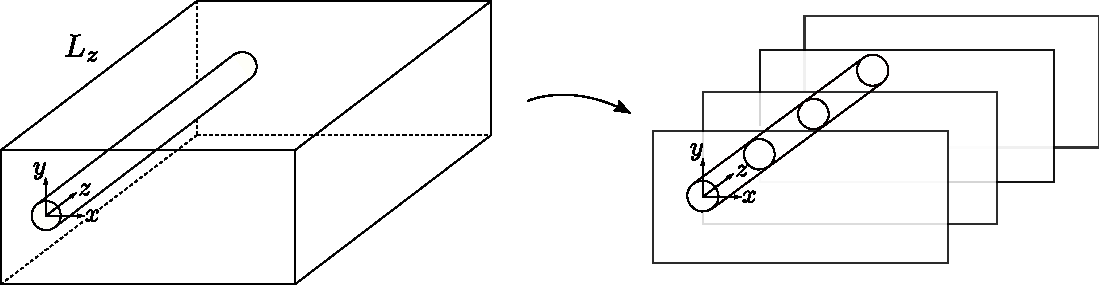
\includegraphics[width=0.9\linewidth]{chapter1/strip_theory_method}
\caption{Sketch of the standard 2-D strip-theory method.
The original $L_z$ span is decomposed into multiple planes in which the 2-D Navier--Stokes equations are solved.}
\label{fig:stm}
\end{figure}

\section{Research objectives and approach}

As exposed in the previous section, current 2-D strip-theory methods lack the inclusion of 3-D physics which have a significant impact on the prediction of flow past long flexible structures.
This motivates the following fundamental questions which have been investigated in this work:
\begin{enumerate}
	\item Why are standard 2-D systems physically not suited for the simulation of flow past long cylinders at high $Re$?
	\item What role does 3-D turbulence play in the wake of a long cylinder and how does it interact with the 2-D K\'{a}rm\'{a}n dynamics?
	\item How can 3-D effects be incorporated and modelled in a 2-D system?
\end{enumerate}

The following investigations have been conducted to provide novel findings on the stated research questions:

\begin{enumerate}
	\item A parametric study of the span effect on the turbulence dynamics of flow past a circular cylinder at $Re=10^4$.
This provides physical understanding on the implications of using 2-D simulations for 3-D turbulent flows and the cross-over between 2-D and 3-D turbulence.
	\item The derivation of a novel 2-D model based on a spanwise-average decomposition of the flow.
This system accounts for 3-D effects and allows to recover the unsteady spanwise-averaged solution of the flow in a 2-D framework.
	\item The design of a machine-learning (ML) model providing closure to the spanwise-averaged system of equations.
\end{enumerate}

\section{Thesis outline and contributions}

The thesis outline and the author's contributions for each chapter is detailed next.
Note that specific literature review is provided in the introductory part of the main content chapters (\cref{chapter:jfm2019}, \cref{chapter:sans} \& \cref{chapter:zanspy}).
Additionally, chapters also include an opening paragraph summarising their specific motivation, conducted research and main findings.

\textit{Chapter 1} provides an introduction to the current work explaining the background and the justification of the thesis.
The research questions and the adopted investigations are specified as well.

\textit{Chapter 2} poses the incompressible flow system of equations and the numerical approach implemented in the in-house solver used throughout this work.

\textit{Chapter 3} analyses the turbulence dynamics in the wake of a circular cylinder at $Re=10^4$ as the span is constricted.
This chapter provides novel results with respect to the domain geometric anisotropy effect on the wake turbulence dynamics in the presence of a solid wall, in contrast with previous studies only considering obstacle-free flows.
\aref{chapter:appendixA} includes information on the phenomena arising in flow past circular cylinder at different Reynolds regimes.
\aref{chapter:appendixB} contains a validation and verification study of the in-house solver for this particular test case.
The initial stage of this work was published in a conference paper for the \textit{OCEANS 2017} meeting.
The complete study has been published in the \textit{Journal of Fluids Mechanics}:

\begin{itemize}
	\item \cite{Font2017} Analysis of two-dimensional and three-dimensional wakes of long circular cylinders. In \textit{OCEANS 2017 - Aberdeen}. IEEE.
	\item \cite{Font2019} Span effect on the turbulence nature of flow past a circular cylinder. \textit{Journal of Fluid Mechanics} \textbf{878}, 306–323
\end{itemize}

\textit{Chapter 4} introduces the spanwise-averaged Navier--Stokes (SANS) equations, a novel 2-D system of equations including 3-D physics through closure terms in the governing equations.
A SANS-based strip-theory framework accounts for 3-D effects otherwise not considered in standard 2-D strip-theory methods, where unphysical dissipative turbulence models are added in order to mitigate their intrinsic limitations.
Additional derivations related to SANS are provided in \aref{chapter:appendixC}.
The perfect closure is evaluated for the Taylor--Green vortex and the circular cylinder cases.
An a-priori assessment of an standard eddy-viscosity model is performed.
This research has been submitted together with \cref{chapter:zanspy}:

\begin{itemize}
	\item \cite{Font2020b} Deep learning the spanwise-averaged Navier--Stokes equations.
\end{itemize}

\textit{Chapter 5} proposes a ML model for the closure of the novel SANS equations.
A-priori and a-posteriori results are shown for the circular cylinder test case, comprising the second part of \cite{Font2020b}.
A generalisation study of the ML model to flow configuration different to the training case is also presented.
Additionally, a hyper-parametric study of the ML model is provided in \aref{chapter:appendixD}, which constitutes a peer-reviewed paper accepted for the \textit{33rd Symposium on Naval Hydrodynamics},

\begin{itemize}
	\item \cite{Font2020a} Turbulent wake predictions using deep convolutional neural networks. In \textit{33rd Symposium on Naval Hydrodynamics}, Osaka, Japan.
\end{itemize}

\textit{Chapter 6} summarises the main findings and limitations as well as future work recommendations.

This research has been presented by the author in the following international conferences:

\begin{itemize}
	\item Font B., Weymouth, G.D., Nguyen, V.-T. \& Tutty, O.R. \href{https://meetings.aps.org/Meeting/DFD19/Session/L17.5}{2019} Deep learning the spanwise-averaged wake of a circular cylinder. \textit{72nd Meeting of the APS Division of Fluid Dynamics}, Seattle, US.

	\item Font B., Elizalde, I., Weymouth, G.D., Nguyen, V.-T. \& Tutty, O.R. \href{https://etc17.fyper.com/program/show_slot/41}{2019} Turbulence dynamics transition of flow past a circular cylinder and the prediction of vortex-induced forces. \textit{European Turbulence Conference 17}, Torino, Italy.

	\item Font B., Weymouth, G.D. \& Tutty, O.R. \href{https://doi.org/10.1109/OCEANSE.2017.8084904}{2017} Analysis of two-dimensional and three-dimensional wakes of long circular cylinders. \textit{OCEANS 2017}, Aberdeen, UK.

	\item Font B., Weymouth, G.D. \& Tutty, O.R. \href{https://www.imperial.ac.uk/media/imperial-college/faculty-of-engineering/aeronautics/UK-Fluids-Conference-2016-booklet.pdf}{2016} A two-dimensional model for three-dimensional symmetric flows. \textit{UK Fluids Conference}, London, UK.
\end{itemize}
% ---------------------------------------------------------------- 
\end{document}